The validation in Section \ref{sec:baseline} identified two structural causes of failure that are independent of any single processing step: a static, content-agnostic slice selection that frequently misses the lesion altogether, and a T2-based hyperintensity criterion that cannot distinguish the tumor from \gls{csf}. The optimized pipeline addresses both causes directly, while reusing the median filtering, \gls{bcet} enhancement, and \gls{fcm} clustering stages of Section \ref{sec:baseline} unchanged.
The proposed optimizations were implemented in order to correct and overcome the two main structural causes:
\begin{itemize}
    \item \textbf{Dynamic slice selection.} Instead of the fixed central slice, the optimal axial slice is determined automatically from the full volume. A single hyperintensity threshold is computed as the 95th percentile of all intracranial voxel intensities in the volume, and the slice containing the largest number of voxels above this threshold is selected. The score is computed entirely from image intensities and never looks at the ground-truth mask, since a real, unlabeled scan would not provide one; an earlier version of this criterion selected the slice with the most ground-truth tumor pixels instead, which is label leakage and was corrected. As a proxy for "the slice most likely to contain the lesion" this criterion is imperfect but unsupervised, and it already reduces the number of patients whose selected slice contains no tumor at all from 39 (8.1\%, Section \ref{sec:baseline}) to 28 (5.8\%).
    \item \textbf{Multimodal transition to \gls{flair}.} The pipeline switches from the T2 to the \gls{flair} channel. \gls{flair} is a T2-weighted inversion-recovery sequence \cite{hajnal1992flair} whose preparation pulse is tuned to null the longitudinal magnetization of free water, physically suppressing the \gls{csf} signal that was identified in Section \ref{sec:baseline} as the dominant confound of the brightest-cluster heuristic. By removing the competing hyperintense structure at the acquisition level, the same intensity-based clustering and cluster-selection logic of the baseline can operate with substantially reduced ambiguity, without requiring any additional topological filter.
    \item \textbf{Dilated ground-truth evaluation.} Manual tumor tracing by a human expert carries an inherent sub-pixel positional uncertainty, and the morphological edge detector of Section \ref{sec:baseline} produces boundaries that are strictly one pixel wide, so that a clinically acceptable prediction offset by a single pixel would otherwise be scored as a complete miss. A tolerance band is therefore introduced by dilating the strict reference boundary with a disk of radius one pixel; $\mathrm{TP}$ is counted whenever a predicted edge pixel falls inside this band, while $\mathrm{FN}$ is still computed against the strict (undilated) boundary, so that $\mathrm{Pnd}$ and Sensitivity reflect the fraction of true boundary actually recovered. \gls{fom}, which already incorporates a continuous distance penalty, is left unchanged and computed on the strict boundary for direct comparability with Section \ref{sec:baseline}.
	\item \textbf{3-D tumor reconstruction (exploratory).} The validated single-slice detection above can be extended into a full 3-D reconstruction of the tumor within the brain volume. A single volume-wide \gls{bcet} enhancement and \gls{fcm} fit ($C=4$) is computed once for the whole brain, rather than refitting per slice, so that cluster assignment is consistent throughout the volume; this volumetric fit is a separate clustering pass used only for the 3-D reconstruction described below, and does not replace or alter the per-slice \gls{fcm} clustering that produces the quantitative results reported in Table \ref{tab:optimized_stats} and Figs. \ref{fig:optimized_pipeline}--\ref{fig:optimized_validation_results}. The lesion is then grown slice-by-slice from the already-validated 2-D detection on the dynamically-selected slice, accepting at each step only the candidate-cluster components overlapping the previously accepted slice; growth stops when the candidate area collapses to a sliver of the seed, or jumps abruptly, signalling that the front has latched onto an unrelated bright structure (e.g. periventricular tissue) rather than continuing the lesion. Fig. \ref{fig:3d_reconstruction} shows the reconstructed brain shell and tumor mass for patient BRATS\_213. Voxel-wise Dice overlap against the 3-D expert ground-truth volumes was computed over all 484 patients: mean $0.315 \pm 0.383$, median $0.044$. The distribution is strongly bimodal: 51 patients (10.5\%) produce a Dice of zero, largely coinciding with cases where the dynamically-selected slice contains no annotated tumor (see Section \ref{sec:optimized}); among the remaining 433 patients, mean Dice reaches $0.352$ and 171 patients (35.3\%) achieve Dice $> 0.5$, including BRATS\_213 (Dice $= 0.63$) and BRATS\_266 (Dice $= 0.78$). The reconstructed volume is systematically larger than the reference on all patients, consistent with the same edema-inclusive over-segmentation already observed at slice level. The high variance mirrors the already-documented spread of the 2-D pipeline (\gls{fom} std $= 0.273$): reconstruction quality is fundamentally bounded by per-patient seed quality, and is presented here as a qualitative extension rather than a clinically validated volumetric segmentation.
	
	\begin{figure}[htbp]
		\centering
		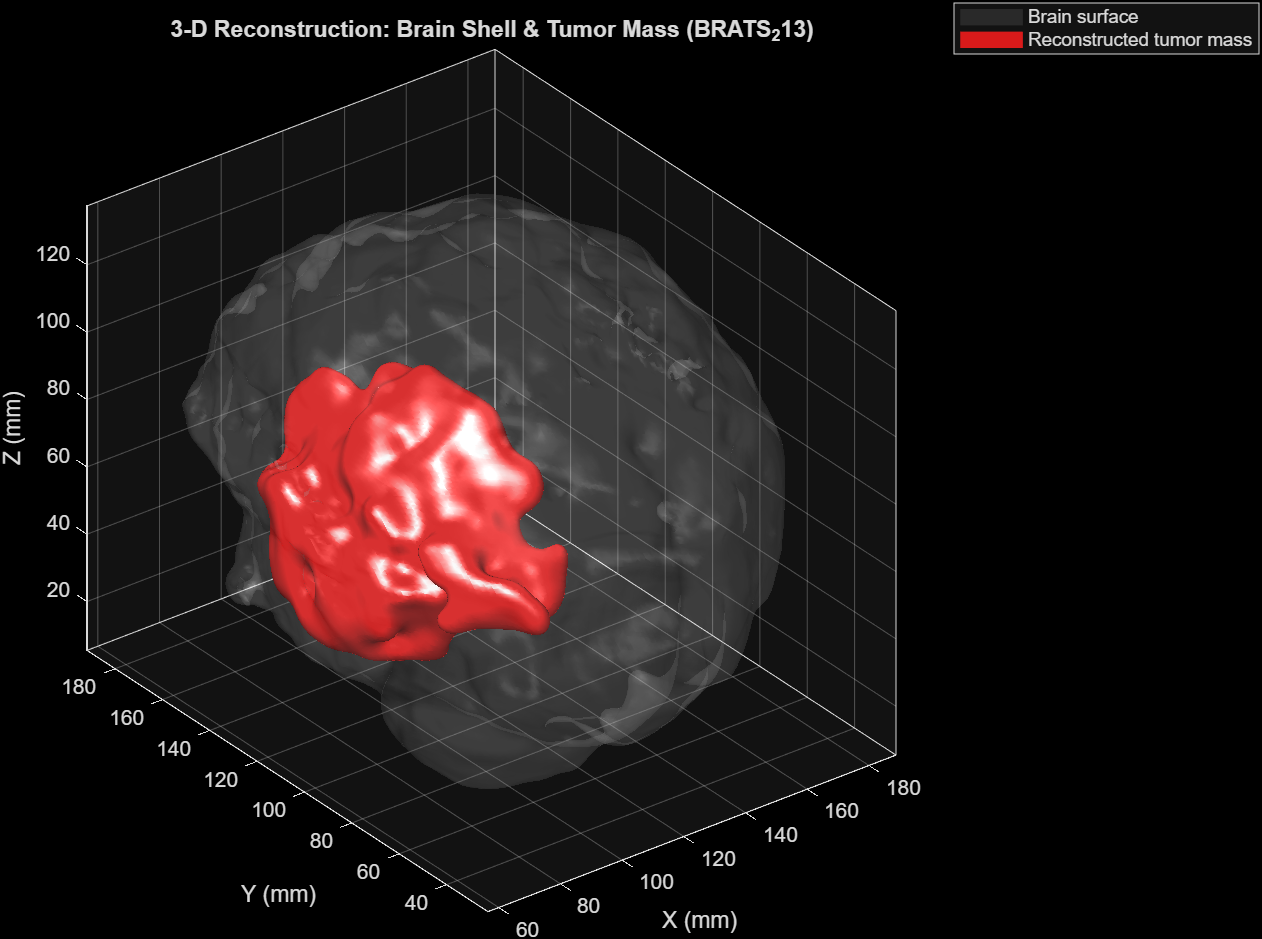
\includegraphics[width=0.9\columnwidth]{images/optimized/best_case/reconstruction.png}
		\caption{3-D reconstruction of patient BRATS\_213: brain surface (translucent gray) and reconstructed tumor mass (red), grown from the validated 2-D detection at the dynamically-selected slice.}
		\label{fig:3d_reconstruction}
	\end{figure}
	
\end{itemize}
Figure \ref{fig:optimized_pipeline} shows the same five stages applied to patient BRATS\_213, the best-\gls{fom} case of the optimized pipeline. The main difference between the optimized pipeline and the baseline is that Panel \ref{fig:optimized_input} shows the \gls{flair} slice selected by the dynamic slice-selection criterion, alongside its ground truth.
\begin{figure}[htbp]
    \captionsetup[subfigure]{justification=centering} 
    \begin{subfigure}[b]{\columnwidth}
        \centering
        
\includegraphics[width=0.9\linewidth]{images/optimized/best_case/01_data_understanding.png}
        \caption[Optimized Input]{normalized FLAIR slice (dynamically selected) and expert-annotated ground truth}
        \label{fig:optimized_input}
    \end{subfigure}
    \vspace{0.1cm}
    \begin{subfigure}[b]{\columnwidth}
        \centering
        
\includegraphics[width=0.9\linewidth]{images/optimized/best_case/02_enhancement.png}
        \caption[Pre-processing]{Pre-processing: median filter, Otsu brain mask, BCET enhancement}
        \label{fig:optimized_preprocessing}
    \end{subfigure}
    \vspace{0.1cm}
    \begin{subfigure}[b]{\columnwidth}
        \centering
        
\includegraphics[width=0.9\linewidth]{images/optimized/best_case/03_segmentation.png}
        \caption{Four-class FCM segmentation and tumor-candidate isolation}
        \label{fig:optimized_segmentation}
    \end{subfigure}
    \vspace{0.1cm}
    \begin{subfigure}[b]{\columnwidth}
        \centering
        
\includegraphics[width=0.9\linewidth]{images/optimized/best_case/04_edge_detection.png}
        \caption{Morphological edge extraction and clinical overlay}
        \label{fig:optimized_edge_extraction}
    \end{subfigure}
    \vspace{0.1cm}
    \begin{subfigure}[b]{\columnwidth}
        \centering
        
\includegraphics[width=0.9\linewidth]{images/optimized/best_case/05_final_validation.png}
        \caption{Validation: predicted boundary vs. expert ground truth}
        \label{fig:optimized_validation}
    \end{subfigure}
    \caption{End-to-end optimized pipeline on patient BRATS\_213 (best FOM case)}
    \label{fig:optimized_pipeline}
\end{figure}
Table \ref{tab:optimized_stats} reports the dataset-wide statistics.
\begin{table}[htbp]
\centering

\caption{Optimized pipeline statistics over 484 BRATS patients.}
\label{tab:optimized_stats}
\begin{tabular}{lcc}
\toprule
Metric & Mean $\pm$ Std & Median \\
\midrule
Sensitivity (Pcd) & $0.248 \pm 0.178$ & $0.241$ \\
\gls{fom} & $0.283 \pm 0.273$ & $0.171$ \\
Accuracy & $0.980 \pm 0.011$ & $0.981$ \\
Pfa & --- & $2.471$ \\
\bottomrule
\end{tabular}
\end{table}

The best, median, and worst cases by \gls{fom} are now patients BRATS\_213 ($\mathrm{FOM}=0.928$), BRATS\_266 ($\mathrm{FOM}=0.171$), and, notably, again BRATS\_012 ($\mathrm{FOM}=0.000$).For this patient, the \gls{flair} hyperintensity criterion selects a different axial slice (Z=43) than the fixed central slice used in the baseline, yet that slice also contains no ground-truth tumor voxels, so neither pipeline detects any reference boundary to compare against. 
\begin{figure}[htbp]
    \centering
    \captionsetup[subfigure]{justification=centering} 
    \begin{subfigure}[b]{\columnwidth}
        \centering
        
\includegraphics[width=0.9\linewidth]{images/optimized/best_case/05_final_validation.png}
        \caption{Best case: BRATS\_213 ($\mathrm{FOM}=0.928$)}
        \label{fig:optimized_best_cases}
    \end{subfigure}
    \vspace{0.1cm} 
    \begin{subfigure}[b]{\columnwidth}
        \centering
        
\includegraphics[width=0.9\linewidth]{images/optimized/median/05_final_validation.png}
        \caption{Median case: BRATS\_266 ($\mathrm{FOM}=0.171$)}
        \label{fig:optimized_median_cases}
    \end{subfigure}
    \vspace{0.1cm}
    \begin{subfigure}[b]{\columnwidth}
        \centering
        
\includegraphics[width=0.9\linewidth]{images/optimized/worst_case/05_final_validation.png}
        \caption{Worst case: BRATS\_012 ($\mathrm{FOM}=0.000$)}
        \label{fig:optimized_worst_cases}
    \end{subfigure}
    \caption{Optimized pipeline comparison between best case \ref{fig:optimized_best_cases}, median case \ref{fig:optimized_median_cases} and worst case \ref{fig:optimized_worst_cases}}
    \label{fig:optimized_validation_results}
\end{figure}
This recurring failure shows that, even though the proposed slice-selection proxy is more reliable on average, it is still a heuristic and gives no guarantee for atypical or very small lesions that do not stand out in the volume-wise hyperintensity statistics. The additional 3-D volume scan required by dynamic slice selection adds little overhead in practice, since computing a percentile and a per-slice voxel count over the volume is cheap compared to the rest of the pipeline: mean processing time per patient rises from 0.99 s for the baseline to 1.06 s for the optimized pipeline, an 8\% increase.
